%
% variationsproblem.tex
%
% (c) 2020 Prof Dr Andreas Müller, Hochschule Rapperswil
%
\begin{frame}
\frametitle{Variationsprobleme}
\begin{columns}[t]
\begin{column}{0.48\hsize}
\begin{block}{Aufgabe}
Gegeben die Funktion $L(t,x,v)$, finde eine Kurve $x(t)$ mit 
$x(a) = x_a$ und $x(b)=x_b$ derart, dass die Wirkung
\[
W
=
W(x)
=
\int_a^b L(t,x(t), \dot x(t))\,dt
\]
minimal ist.
\end{block}
\end{column}
\begin{column}{0.48\hsize}
\begin{center}
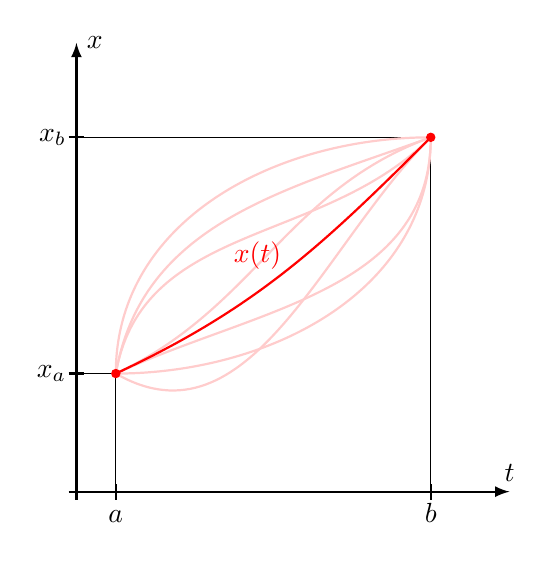
\begin{tikzpicture}[>=latex,thick]

\coordinate (A) at (0.5,1.5);
\coordinate (B) at (4.5,4.5);

\draw[line width=0.5pt] (0.5,0)--(A)--(0,1.5);
\draw[line width=0.5pt] (4.5,0)--(B)--(0,4.5);

\draw (-0.1,4.5)--(0.1,4.5);
\draw (-0.1,1.5)--(0.1,1.5);
\node at (0,1.5) [left] {$x_a$};
\node at (0,4.5) [left] {$x_b$};

\draw[->] (-0.1,0)--(5.5,0) coordinate[label={$t$}];
\draw[->] (0,-0.1)--(0,5.7) coordinate[label={right:$x$}];
\draw (0.5,-0.1)--(0.5,0.1); \node at (0.5,0) [below] {$a\mathstrut$};
\draw (4.5,-0.1)--(4.5,0.1); \node at (4.5,0) [below] {$b\mathstrut$};

\draw[color=red!20] (A) to[out=0,in=-90] (B);
\draw[color=red!20] (A) to[out=-30,in=-135] (B);
\draw[color=red!20] (A) to[out=25,in=-90] (B);
\draw[color=red!20] (A) to[out=80,in=-160] (B);
\draw[color=red!20] (A) to[out=25,in=-160] (B);
\draw[color=red!20] (A) to[out=80,in=-135] (B);
\draw[color=red!20] (A) to[out=90,in=-180] (B);

\draw[color=red] (A) to[out=25,in=-135] (B);
\fill[color=red] (A) circle[radius=0.06];
\fill[color=red] (B) circle[radius=0.06];

\node[color=red] at (2.3,3) {$x(t)$};

\end{tikzpicture}
\end{center}
\end{column}
\end{columns}
\end{frame}
